\chapter{Materiais e Métodos}

Esta seção descreve as etapas do desenvolvimento da API, assim como a aplicação e utilização das ferramentas e suas tecnologias. Este desenvolvimento foi realizado utilizando a generalização de conceitos de engenharia de software, com o objetivo de gerar desacoplamento e reutilização de código. As etapas de desenvolvimento se deram através das etapas necessárias para a construção de uma API REST e organizadas utilizando a metodologia ágil Kanban.

\section{Bibliotecas e Ferramentas}

A escolha das bibliotecas e softwares deste projeto, devem-se a pesquisas que tiveram como foco: 
\begin{itemize}
    \item Suporte dos desenvolvedores: Dada a necessidade de se ter uma ferramenta que seja confiável e atualizada.
    \item Alta utilização pela comunidade: Já que a maioria destas ferramentas são de código livre e podendo a comunidade submeter melhorias e realizar fiscalização do que está sendo alterado na mesma.
    \item Compatibilidade a outros componentes e estrutura do projeto: Um dos objetivos deste software é que ele seja mutável, para que de acordo com as mudanças que podem ocorrer em outras tecnologias e estruturas de documentos PDF, esteja apto a acompanhar tais alterações.
\end{itemize}

\subsection{PDF.JS - v2.2.228}

O PDF.JS, criado em 2011 pela Mozilla Foundation, é uma biblioteca amplamente utilizada, e se encontra presente na maioria dos websites que fazem qualquer tipo de manipulação e exibição de PDF. Esta foi criada como uma extensão do navegador Firefox, com a intenção de renderizar arquivos PDF, de forma rápida e segura, no navegador do cliente. Apesar da migração de uma biblioteca específica para o navegador da Mozilla, seu formato de renderização permanece o mesmo, onde ela acessa a estrutura do arquivo PDF, coleta o conteúdo e a formatação no \textit{Body}, realiza a conversão para HTML e CSS de cada objeto encontrado e com a tabela XREF o arquivo é remontado no navegador do cliente como um PDF dentro da página.

Com a evolução das tecnologias e a busca contínua por melhor performance, esta biblioteca conta com centenas de funções e diferentes abordagens para e leitura das mais variadas formas de PDF. Utilizando o resultado destas funções, é possível realizar extrações para coleta de informações encontradas no arquivo, informações como o texto puro, posição de elementos na página, fonte utilizada, cor e vários outros tipos.

Como o objetivo deste sistema está diretamente ligado a extração dos dados e o foco principal desta biblioteca é a renderização do arquivo no navegador, boa parte das funções mais pesadas nesta biblioteca não são necessárias.

\subsection{Extract - v0.1.3}
Convenientemente, há um módulo criado pela comunidade que encapsula somente a parte e extração de dados contida na biblioteca e entrega de forma leve e prática todas as funcionalidades necessárias para uma boa extração do conteúdo do arquivo PDF.

Fundamentalmente, a leitura acontece de forma que, dado o caminho do arquivo e um objeto de opções, onde podem ser especificadas quais páginas deve ser lidas, a formatação dos espaços entre outro, são extraídos metadados do arquivo como o autor, o software utilizado para salvar o arquivo, o software utilizado para gerar o PDF, última data de edição entre outros. Junto ao objeto de metadados é retornado um vetor contendo um objeto JSON para cada página analisada, este objeto contém todas as informações básicas necessária para análise do conteúdo como é possível ver  \textbf{Figura \ref{pdfExtract}}

\begin{figure}
\centering
\captionsetup{justification   = raggedright,
              singlelinecheck = false}
\caption{Objeto JSON após extração de informação de um PDF através da biblioteca Extract}\label{pdfExtract}
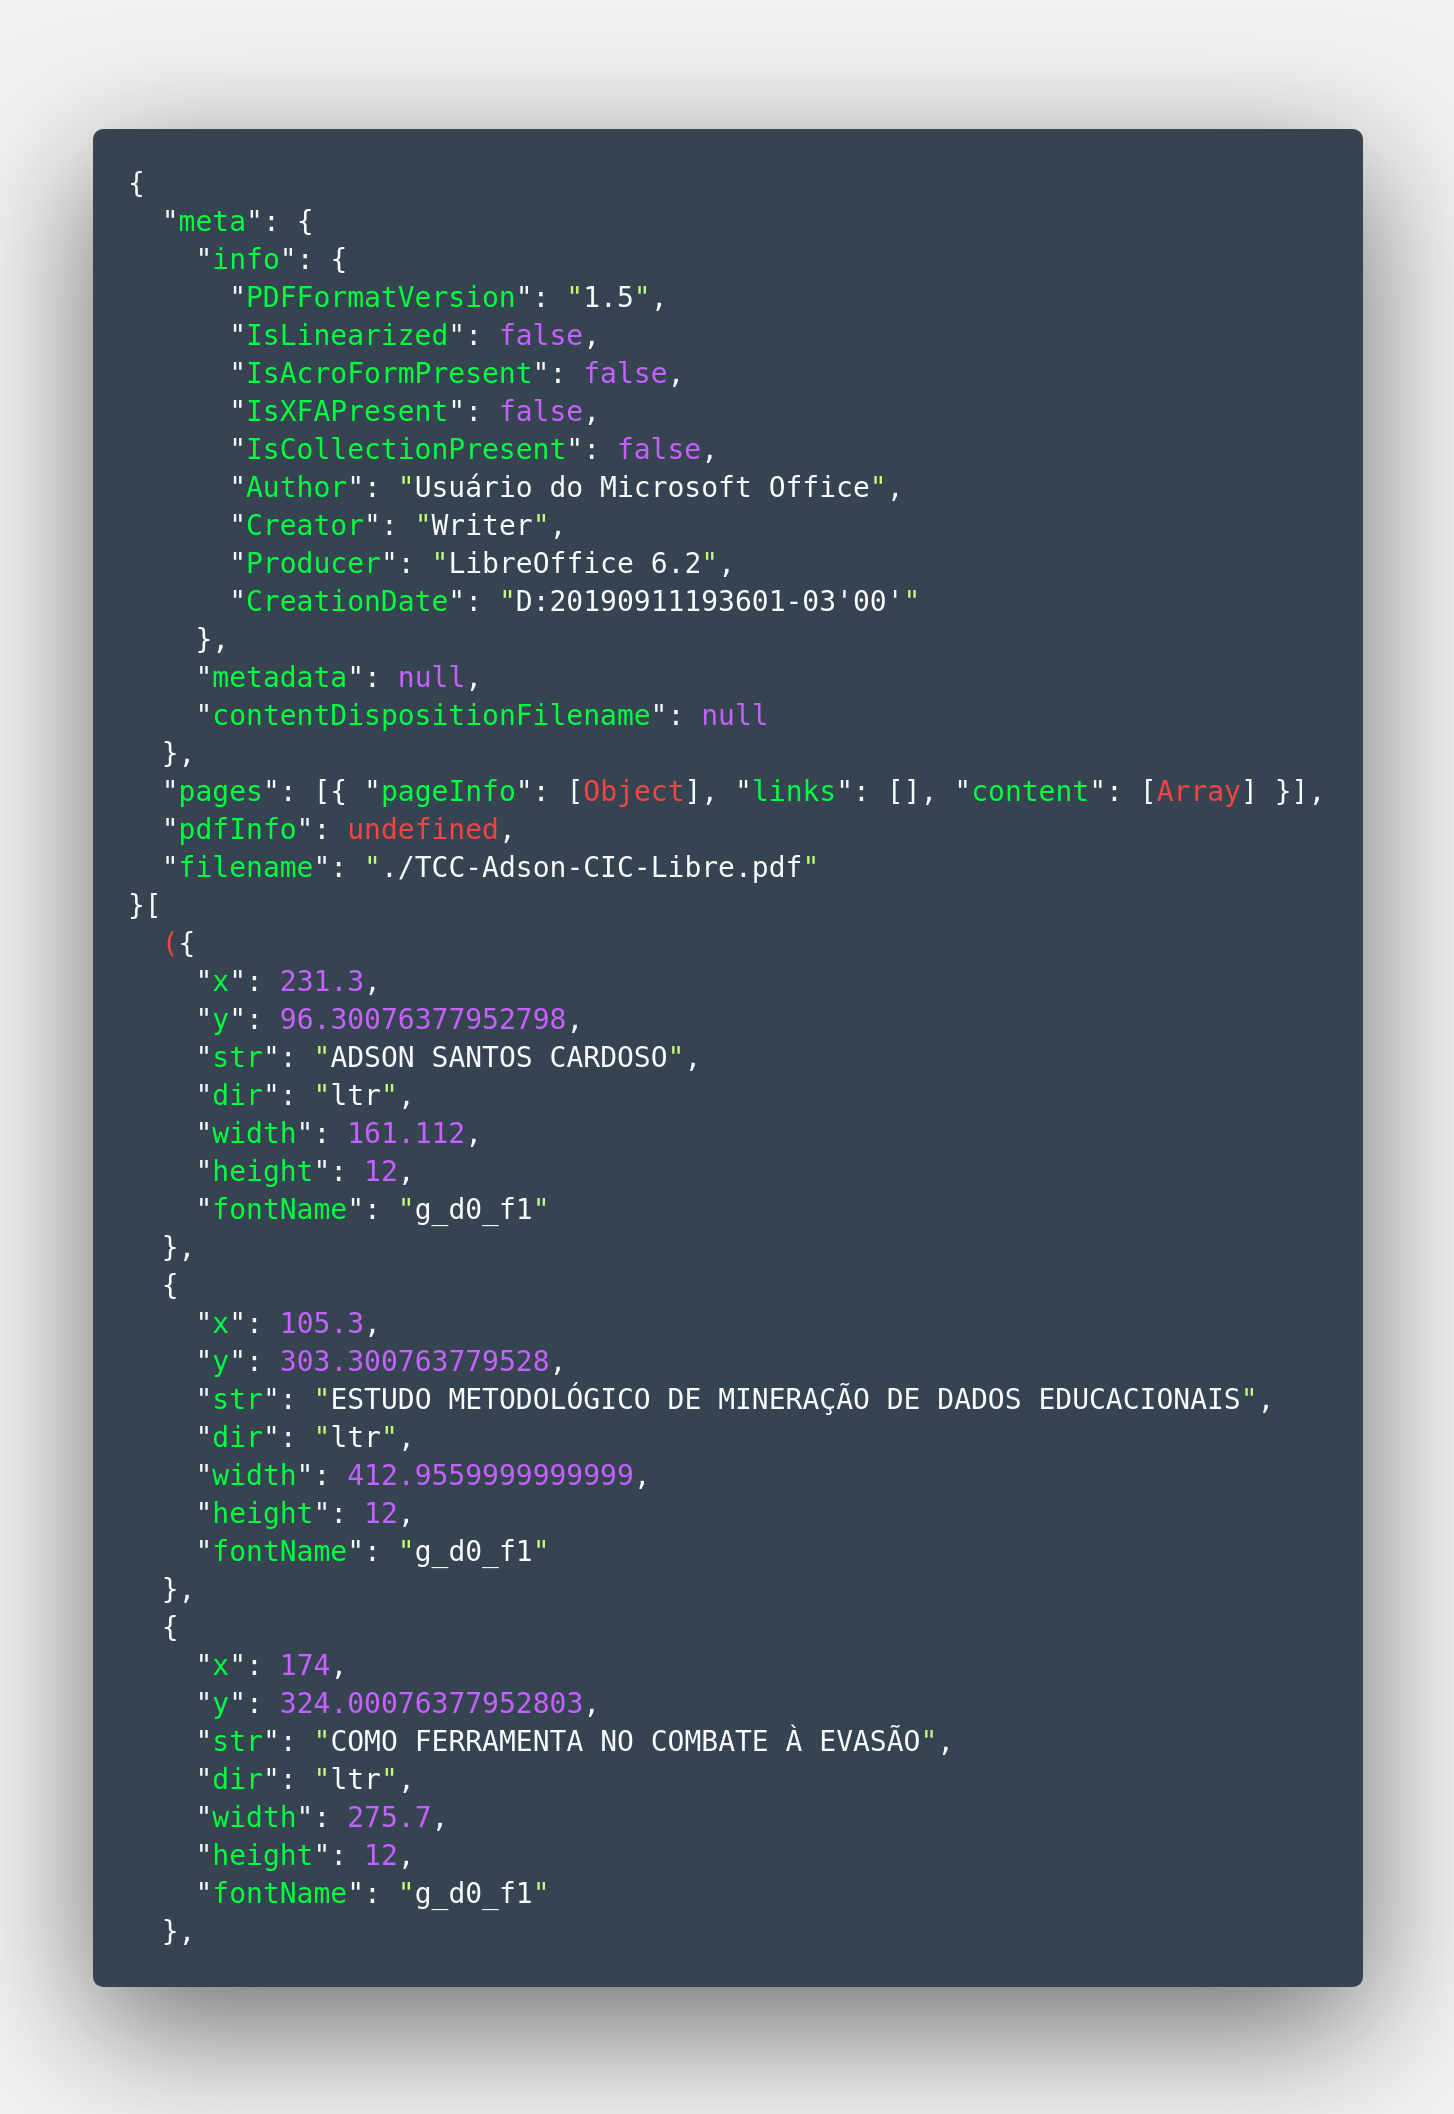
\includegraphics[width=0.8\textwidth]{figs/pdfExtract.png}
\end{figure}

Após extrair essas informações o próximo passo foi a filtragem deste conteúdo.

\subsection{Extract By Coord}

Dado o objetivo de extrair a informação dado um espaço da página, definido por coordenadas X e Y, foi feita uma pesquisa de formas práticas para se realizar a filtragem do conteúdo, por tais coordenadas, assim foi encontrada uma pequena biblioteca no GitHub, com a licença MIT, que realizava uma abordagem similar a necessária para a próxima etapa da extração dos dados.

Esta biblioteca oferece duas funcionalidades, a primeira encapsula a extração feita pela biblioteca Extract, com o intuito de descartar informações desnecessárias para a análise, como a rotação, escala, tamanho da página, e evidenciar o software responsável por gerar o arquivo PDF, a importância desta informação será detalhada no tópico X. Além disso, os objetos na página são ordenados da esquerda a direita e de cima para baixo, e selecionado apenas os dados de coordenadas e string. Desta forma é retornado um objeto JSON enxuto, contendo apenas as informações necessárias e pronto para ser recebido como entrada da segunda função. 

Esta função é responsável por extrair o conteúdo, ela recebe o nome do programa responsável por gerar o arquivo PDF, a importância deste valor é decorrente da forma que diferentes programas atribuem diferentes formas de espaçamento entre as strings, por exemplo o Microsoft Word realiza o espaçamento dos objetos atribuindo vários objetos de espaço, além disso são recebidos o objeto da página a ser extraída, e as coordenadas X e Y de início e de fim como objeto JSON. Ao ser executada, são observadas as coordenadas de cada objeto dentro da página, estando no alcance das coordenadas recebidas, sua string é extraída e tratada, de acordo com o software que gerou o arquivo PDF. Desta forma é retornada uma string com o que se encontra naquela região.

Esta biblioteca foi alterada para que o texto recebido fosse entregue com uma formatação correta, devido a diferença de espaços causada pelo software que gerou o PDF, além disso foi feita uma melhor filtragem pelo sistema de coordenadas e a função de extração passou a aceitar mais de uma página.

\subsection{RegEx - Expressão Regular}
O RegEx, derivado da expressão regular definida na teoria da computação, entrega uma forma de se identificar cadeia de caracteres, dada uma expressão regular em linguagem formal. Ou seja, dada uma expressão é possível encontrar cadeias que aceitem tais condições. A linguagem JavaScript carrega todo um grupo de funções que auxiliam na utilização de expressões regulares, assim não é necessária nenhuma biblioteca adicional.

Como forma de limitação ou busca de valor específico são utilizadas expressões regulares que tanto removem trechos que podem afetar a busca de um valor, quanto encontram um valor específico após determinada palavra. Como por exemplo no caso de haver um Coorientador quando se está um busca do nome do Orientador, então é feita a busca pelo Coorientador e se encontrado seu valor é retirado, isso ocorre devido a utilização da expressão regular com \textit{lookbehind}(olhar atrás), já que o valor buscado está depois da palavra Orientador, então retirar o Coorientador serve como uma condição de parada, assim como pontuação e quebra de linha.

A filtragem com o RegEx assegura o conteúdo encontrado e delimita a informação buscada, no caso de ocorrer um bloco inesperado dentro das coordenadas. 

\subsection{JWT - \textit{JSON Web Token} (v8.5.1) }

Com a necessidade de se ter uma forma de autenticação segura e prática, foi optado pela utilização do \textit{JSON Web Token}. Comumente, o desenvolvedor realiza a implementação de seu próprio método de autenticação, porém, segundo a \textit{Open Web Application Security Project} (OWASP), uma organização sem fins lucrativos que trabalha em prol da segurança na web, buscando falhas e formas de combater as mesmas, a “Quebra de Autenticação e Gerenciamento de Sessão” é um dos maiores e mais recorrentes problemas em aplicações web. A falta de uma boa criptografia e métodos seguros de envio e recebimento de dados ocasiona oportunidades para que usuários mal intencionados consigam invadir contas e ter acesso a informações sigilosas.

O JWT é um padrão aberto (RFC 7519), que define de forma compacta, independente e segura, um método de transmitir informações como objeto JSON. Sendo uma forma segura, com bibliotecas para a maioria das linguagens utilizadas na web e suporte nativo do JSON nos navegadores modernos,  o JWT se tornou a escolha ideal como método de autenticação. 

Utilizando o algoritmo HMAC \textit{(Hash based Message Authentication Code)}, a informação é encriptada com um segredo que apenas o lado do servidor contém, (também podem ser utilizados pares de chaves pública/privada através da encriptação por RSA ou ECDSA), e passada como um cabeçalho HTTP. Desta forma, quando o usuário realiza uma requisição, o servidor chama um método de validação do \textit{token} (\cite{jwt}).

\subsection{MongoDB}

O MongoDB é um banco de dados não relacional, onde os dados são armazenados em documentos JSON, por isso é dito que este é um banco orientado a documentos. Desta forma não há necessidade da criação de tabelas e colunas na fase de modelagem do banco, assim há uma liberdade maior para que o documento que será salvo represente apenas as informações necessárias e suas relações não sejam pré definidas.

Esta flexibilidade é de grande ajuda quando se trata de uma aplicação que pode mudar a organização e o tipo de informação a ser salva, diferente de um banco relacional, onde toda sua estrutura deveria ser mudada para que se adequasse a estas mudanças. No caso dessa aplicação, o usuário irá definir quais informações serão extraídas do PDF e assim o objeto JSON com as informações será montado, além disso o usuário também tem a liberdade de adicionar ou remover um campo de informação a ser extraída ou adicionar um novo sem afetar a estrutura do banco.

A escolha do MongoDB entre os bancos não relacionais foi feita devido a sua alta performance, facilidade de manipulação em relação a sua infraestrutura, popularidade e principalmente a biblioteca Mongoose. 

\subsubsection{Mongoose}

O manipulação do Mongo foi feita através da biblioteca Mongoose, onde a modelagem de dados é baseada em esquemas. Ao realizar uma consulta ao banco de dados, através do mongoose, é realizada conversão do dado para um objeto JavaScript, assim quando recuperada uma informação do banco, sua manipulação se torna algo simples e orgânico no fluxo de desenvolvimento. Também é possível realizar validações através da declaração do esquemas, isso impõe mais uma camada de segurança entre o usuário e a API. 

\section{Metodologia e Desenvolvimento}

Neste tópico, serão explicados como cada ferramenta, definida no tópico anterior foi utilizada. Os detalhes mais específicos podem ser encontrados no repositório deste projeto no GitHub, publicamente aberto e é possível enviar mudanças para que sejam avaliadas e incorporadas no código. Também será descrito como foi modelada a estrutura deste sistema e dividia as etapas de desenvolvimento.

\subsection{Metodologia Ágil}

Para a organização e definição das tarefas que objetivam a completude deste projeto foi escolhida a metodologia ágil Kaban. Criado pela Toyota nos anos 70, o Kanban (que pode ser traduzido como Cartão),  sinalizava a disponibilidade para se trabalhar em uma peça, quando se fazia necessário para outras etapas da produção. Dessa forma havia uma maior organização na ordem de trabalho, não havia desperdício de peças e através dos cartões era possível ver o progresso geral.

Com estas vantagens é possível aplicar ao desenvolvimento de software o Kanban e trazer até mais algumas vantagens ao fluxo de trabalho para a programação. 
Aplicando esta metodologia é feito um quadro consistente de três colunas, uma de tarefas \textbf{A fazer}, em seguida as tarefas \textbf{Em andamento} e finalizando com as tarefas \textbf{Concluídas}.

O GitHub oferece uma implementação do Kanban, diretamente no repositório para que outros colaboradores possam interagir e a visualização e utilização sejam práticas.

Foram separados por ordem de prioridade as tarefas necessárias para atingir a completude da API, e adicionadas nas lista de A fazer no kanban, foram priorizadas aquelas que eram necessárias para o funcionamento e teste da API, assim foi feito uma por vez até que houvessem mais tarefas que impedissem o funcionamento de tal.

\subsection{MVC - \textit{Model View Controller}}

A estrutura deste sistema foi elaborada de acordo com o padrão de desenvolvimento MVC,